% !TeX root=abs_formeln.tex

\subsection{Stromstärke}
\begin{equation}\label{eq:elektrischer:strom}
I = \frac{\Delta Q}{\Delta t}
\end{equation}

\begin{equation}\label{eq:elektrischer:strom:elektronen}
I = \frac{n \cdot e \cdot v}{\Delta s}
\end{equation}

\subsection{Elektrische Feldstärke}
\begin{equation}\label{eq:elektrische:feldstaerke}
E = \frac{F}{q}
\end{equation}

\subsection{Bifilares Plättchen im elektrischen Feld}
\begin{equation}\label{eq:bifilares:plaettchen:1}
F = F_G \cdot \frac{s}{h}
\end{equation}

\begin{equation}\label{eq:bifilares:plaettchen:2}
F \approx F_G \cdot \frac{s}{\ell}
\end{equation}

\subsection{Elektrische Spannung}
\begin{equation}\label{eq:elektrische:spannung}
U = \frac{W}{q}
\end{equation}

\begin{equation}\label{eq:elektrische:spannung:feld}
U = E \cdot d
\end{equation}

\subsection{Ohmsches Gesetz}
\begin{equation}\label{eq:ohmsches:gesetz}
U = R \cdot I
\end{equation}

\subsection{Spezifischer Widerstand}
\begin{equation}\label{eq:spezifischer:widerstand}
R = \varrho\cdot\frac{\ell}{A}
\end{equation}

\subsection{Elektrische Energie}
\begin{equation}\label{eq:elektrische:energie}
W = U \cdot I \cdot t
\end{equation}

\subsection{Elektrische Leistung}
\begin{equation}\label{eq:elektrische:leistung}
P = \frac{W}{t} = U \cdot I
\end{equation}

\subsection{Reihenschaltung von Widerständen}
\begin{equation}\label{eq:widerstand:reihenschaltung:spannung}
U = U_1 + U_2 
\end{equation}

\begin{equation}\label{eq:widerstand:reihenschaltung:strom}
I = I_1 = I_2
\end{equation}

\begin{equation}\label{eq:widerstand:reihenschaltung:widerstand}
R = R_1 + R_2
\end{equation}

\subsection{Parallelschaltung von Widerständen}
\begin{equation}\label{eq:widerstand:parallelschaltung:spannung}
U = U_1 = U_2
\end{equation}

\begin{equation}\label{eq:widerstand:parallelschaltung:strom}
I = I_1 + I_2
\end{equation}

\begin{equation}\label{eq:widerstand:parallelschaltung:widerstand}
\frac{1}{R} = \frac{1}{R_1} + \frac{1}{R_2} 
\end{equation}

\subsection{Elektrisches Potential}
\begin{equation}\label{eq:elektrisches:potential}
\Delta \varphi = \varphi_2 - \varphi_1
\end{equation}

\subsection{Flächenladungsdichte}
\begin{equation}\label{eq:flaechenladungsdichte}
\sigma = \frac{Q}{A}
\end{equation}

\begin{equation}\label{eq:flaechenladungsdichte:feld}
\sigma = \varepsilon_0 \cdot \varepsilon_r \cdot E
\end{equation}

\subsection{Coulomb-Gesetz}
\begin{equation}\label{eq:coulomb:gesetz}
F = q \cdot E = \frac{1}{4\cdot \pi \cdot \varepsilon_0}\cdot \frac{Q \cdot
 q}{r^2}
\end{equation}

\subsection{Coulomb-Potential}
\begin{equation}\label{eq:coulomb:potential}
\varphi = \frac{1}{4\cdot \pi \cdot \varepsilon_0}\cdot \frac{Q}{r}
\end{equation}

\begin{equation}\label{eq:coulomb:potential:energie}
W_{12} = \frac{Q \cdot q}{4\cdot \pi \cdot
 \varepsilon_0}\cdot\left(\frac{1}{r_1} - \frac{1}{r_2}\right)
\end{equation}

\begin{equation}\label{eq:coulomb:potential:spannung}
U_{12} = \frac{Q}{4\cdot \pi \cdot
 \varepsilon_0}\cdot\left(\frac{1}{r_1} - \frac{1}{r_2}\right)
\end{equation}

\subsection{Kondensatoren}
\begin{equation}\label{eq:kondensator:kapazitaet}
C = \frac{Q}{U}
\end{equation}

\begin{equation}\label{eq:kondensator:kapazitaet:platten}
C = \varepsilon_0 \cdot \varepsilon_r \cdot \frac{A}{d}
\end{equation}

\subsection{Kugelkondensator}
\begin{equation}\label{eq:kondensator:kapazitaet:kugel}
C = \frac{4\cdot\pi\cdot\varepsilon_0}{\frac{1}{r_1}-\frac{1}{r_2}}
\end{equation}

\subsection{Reihenschaltung von Kondensatoren}
\begin{equation}\label{eq:kondensator:reihenschaltung:ladung}
Q = Q_1 = Q_2
\end{equation}
 
\begin{equation}\label{eq:kondensator:reihenschaltung:spannung}
U = U_1 + U_2 
\end{equation}
 
\begin{equation}\label{eq:kondensator:reihenschaltung:kapazitaet}
\frac{1}{C} = \frac{1}{C_1} + \frac{1}{C_2}
\end{equation}

\subsection{Parallelschaltung von Kondensatoren}
\begin{equation}\label{eq:kondensator:parallelschaltung:ladung}
Q = Q_1 + Q_2
\end{equation}

\begin{equation}\label{eq:kondensator:parallelschaltung:spannung}
U = U_1 = U_2
\end{equation}

\begin{equation}\label{eq:kondensator:parallelschaltung:kapazitaet}
C = C_1 + C_2
\end{equation}

\subsection{Kondensatorentladung}
\begin{equation}\label{eq:kondensator:entladung:zeit}
T_H = \SI{0.69}{} \cdot R \cdot C
\end{equation}

\begin{equation}\label{eq:kondensator:entladung:spannung}
U(t) = U_0 \cdot 2^{-\frac{t}{T_H}}
\end{equation}

\begin{equation}\label{eq:kondensator:entladung:ladung}
Q(t) = Q_0 \cdot 2^{-\frac{t}{T_H}}
\end{equation}

\begin{equation}\label{eq:kondensator:entladung:strom}
I(t) = I_0 \cdot 2^{-\frac{t}{T_H}}
\end{equation}

\subsection{Energie eines geladenen Kondensators}
\begin{equation}\label{eq:kondensator:energie:spannung}
W = \frac{1}{2} \cdot C \cdot U^2
\end{equation}

\begin{equation}\label{eq:kondensator:energie:feld}
W = \frac{1}{2} \cdot \varepsilon_0 \cdot \varepsilon_r \cdot E^2 \cdot V
\end{equation}

\subsection{Räumliche Dichte der elektrischen Energie}
\begin{equation}\label{eq:rauemliche:dicht:elektrische:energie}
\varrho_{el} = \frac{W}{V} = \frac{1}{2} \cdot \varepsilon_0 \cdot \varepsilon_r \cdot
 E^2
\end{equation}

\subsection{Anziehungskraft zwischen zwei Kondensatorplatten}
\begin{equation}\label{eq:kondensator:anziehungskraft}
F = \frac{\Delta W}{\Delta s}
\end{equation}

\begin{equation}\label{eq:kondensator:anziehungskraft:elektrisches:feld}
F = \frac{1}{2}\cdot\varepsilon_0 \cdot
\varepsilon_r \cdot E^2 \cdot A
\end{equation}

\begin{equation}\label{eq:kondensator:anziehungskraft:spannung}
F = \frac{1}{2}\cdot\varepsilon_0 \cdot \varepsilon_r \cdot
 \frac{U^2}{d^2} \cdot A
\end{equation}

\subsection{Magnetische Flussdichte}
\begin{equation}\label{eq:magnetische:flussdichte}
B = \frac{F}{I \cdot s}
\end{equation}

\begin{equation}\label{eq:magnetische:flussdichte:schlanke:spule}
B = \mu_0 \cdot \mu_r \cdot \frac{n}{\ell} \cdot I
\end{equation}

\begin{equation}\label{eq:magnetische:flussdichte:relative:permeabilitaet}
\mu_r = \frac{B_m}{B_0}
\end{equation}

\subsection{Lorentzkraft}
\begin{equation}\label{eq:lorentzkraft}
F_L = Q \cdot v_s \cdot B
\end{equation}

\subsection{Hall-Spannung}
\begin{equation}\label{eq:hall:spannung}
U_H = B \cdot v_s \cdot h
\end{equation}

\subsection{Magnetfeld der Erde}
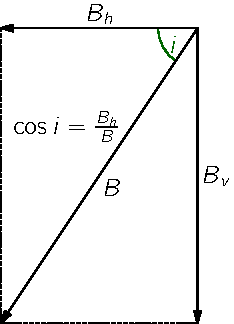
\includegraphics[width=.4\linewidth]{magnetfeld_der_erde} \hfill
\begin{minipage}[b]{.55\linewidth}\raggedright
Inklinationswinkel: $i$

Horizontalkomponente des Erdmagnetfelds: $B_h$

Vertikalkomponente des Erdmagnetfelds: $B_v$
\end{minipage}

\subsection{Ladungen im Magnetfeld}
\begin{equation}\label{eq:magnetfeld:elektronen:kreisbahn}
r = \frac{v_s \cdot m}{B \cdot q}
\end{equation}

\subsection{Magnetische Induktion}
Anzahl der Leiterschleifen: $n$

$A_s$ ist die senkrecht von den Feldlinien durchsetzte Fläche. Sie ist mit Hilfe der trigonometrischen Funktionen aus A berechenbar.
 
\subsubsection{durch Leiterbewegung}
\begin{equation}\label{eq:magnetische:induktion:leiterbewegung}
U_{ind} = n \cdot B \cdot d \cdot v_s
\end{equation}

\subsubsection{durch Flächenänderung}
\begin{equation}\label{eq:magnetische:induktion:flaechenaenderung}
U_{ind} = n \cdot B \cdot d \cdot v_s = n \cdot B \cdot \frac{\Delta A_s}{\Delta t}
\end{equation}

\subsubsection{durch Drehung}
\begin{equation}\label{eq:magnetische:induktion:drehung}
U_{ind} = n \cdot B \cdot \frac{\Delta A_s}{\Delta t}
\end{equation}

\subsubsection{durch Flussdichteänderung}
\begin{equation}\label{eq:magnetische:induktion:flussdichteaenderung}
U_{ind} = n \cdot A_s \cdot \frac{\Delta B}{\Delta t}
\end{equation}
  
\subsubsection{durch Änderung des magnetischen Flusses}
\begin{equation}\label{eq:magnetische:induktion:flussaenderung}
U_{ind}(t) = n \cdot \frac{\Delta \Phi}{\Delta t}
\end{equation}

\subsubsection{Momentanspannung für $\Delta t \to 0$}
\begin{equation}\label{eq:magnetische:induktion:momentanspannung}
U_{ind}(t) = n \cdot \dot{\Phi}(t)
\end{equation}

\subsection{Magnetischer Fluss}
\begin{equation}\label{eq:magnetischer:fluss}
\Phi = B \cdot A_s
\end{equation}

\subsection{Selbstinduktion einer Spule}
\begin{equation}\label{eq:spule:selbstinduktion}
U_{ind}(t) = - n \cdot \dot{\Phi}(t) = - L \cdot \dot{I}(t)
\end{equation}
\begin{equation}\label{eq:spule:induktivitaet}
L = \mu_0\cdot
\mu_r \cdot n^2 \cdot \frac{A}{\ell}
\end{equation}